\documentclass[
letterpaper,
11pt,
oneside,
twocolumn, %twocolumn para dos columnas
article
]{memoir}

\usepackage[spanish,es-nodecimaldot]{babel}
\usepackage[utf8]{inputenc}
\usepackage[T1]{fontenc}
\usepackage{tgtermes} % La fuente a usar, si no compila quitar esta línea
\medievalpage

% Paquetes para matemáticas
\usepackage{amscd}
\usepackage{amsfonts}
\usepackage{amssymb}
\usepackage{amsmath}
\usepackage{amsthm}
\usepackage{latexsym}
\usepackage{mathrsfs}
\usepackage{bm}
\usepackage{bbm}
\usepackage{mathtools}

\usepackage[final]{microtype}
\usepackage{graphicx} % Para incluir figuras
\usepackage{lipsum}

\usepackage{hyperref}

\setlrmarginsandblock{0.1\paperwidth}{*}{1} % Para twocolumn
\setulmarginsandblock{1.5in}{2in}{1}  % Márgenes superior e inferior
\checkandfixthelayout

\addto{\captionsspanish}{%
  \renewcommand{\bibname}{\Large Referencias}
}

\counterwithout{section}{chapter}
\counterwithout{figure}{chapter}

\makeatletter
\def\@maketitle{%
  \newpage
  \null
  \vskip 2em%
  \let \footnote \thanks
  \begin{center}
    {\LARGE \textsc \@title \par}%
    \vskip 0.5em%
    {\large Procesos Estocásticos I \par}
    \vskip 0.5em%
    {\large
      \lineskip .5em%
      \begin{tabular}[t]{c}%
        \@author
      \end{tabular}\par}%
    \vskip 1em%
    %{\large \@date}%
  \end{center}
  \par
  \vskip 1.5em}
\makeatother

\makepagestyle{plain}
\makeevenfoot{plain}{\thepage}{}{}
\makeoddfoot{plain}{}{}{\thepage}
\makeevenhead{plain}{}{}{}
\makeoddhead{plain}{}{}{}

\title{Título del reporte} % Cambiar título
\author{Nombre del alumno} % Su nombre

\begin{document}
\thispagestyle{empty}
\maketitle

\begin{abstract}
    Si quieren poner un lindo resumen o qué sé yo. Si prefieren no resumir su trabajo (que debería de ser de unas cuantas páginas, borrar estas líneas.
\end{abstract}

\epigraph{Aquí pueden poner alguna cita que les guste}{Su autor preferido}

\section*{Sección 1}

\noindent El primer párrafo va sin sangría.\footnote{Nota al pie de página} Matemáticas dentro del texto $x = y$ y ecuaciones que tienen su propias línea \[\int f (x) \mu(d x).\] 

\lipsum[1-6]

\section*{Otra sección}

\noindent Aquí va otra sección. Si quieren agregar una imagen como en la figura \ref{Figura}, se usa el comando \texttt{\textbackslash{}includegraphics}.

\begin{figure}[ht]
    \centering
    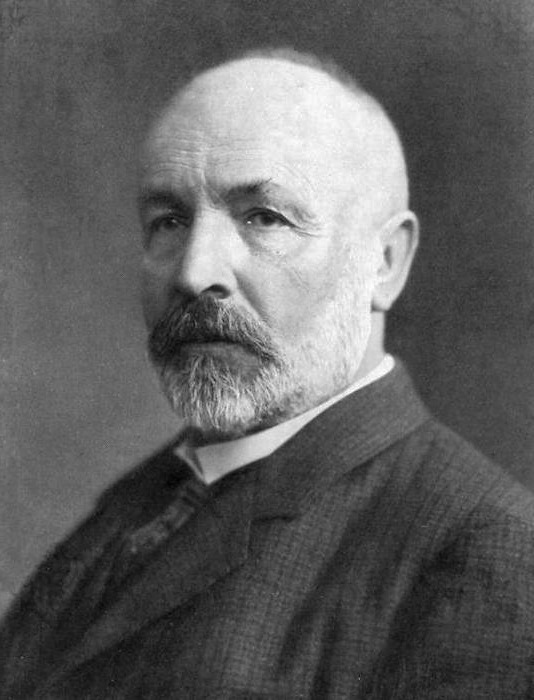
\includegraphics[width=0.3\textwidth,keepaspectratio]{Cantor}
    \caption{Nadie nos podrá sacar del paraíso que ha creado.}
    \label{Figura}
\end{figure}

Pasemos a la bibliografía, la cual pueden citar con \texttt{\textbackslash{}cite}: \cite{latexcompanion}, \cite{einstein}, \cite{knuthwebsite}.

\begin{thebibliography}{9}
\bibitem{latexcompanion} 
Michel Goossens, Frank Mittelbach, and Alexander Samarin. 
\textit{The \LaTeX\ Companion}. 
Addison-Wesley, Reading, Massachusetts, 1993.
 
\bibitem{einstein} 
Albert Einstein. 
\textit{Zur Elektrodynamik bewegter K{\"o}rper}. (German) 
[\textit{On the electrodynamics of moving bodies}]. 
Annalen der Physik, 322(10):891–921, 1905.
 
\bibitem{knuthwebsite} 
Knuth: Computers and Typesetting.
\end{thebibliography}

\end{document}
